%#!platex main

\chapter{実行時環境}
\label{083441_12Apr06}
% 7.3節まで

以降の章では、意味解析部までで得られた解析木をもとに機械語命令列を生成す
る部分({\bf コード生成部})について説明を行う。

実際に生成される機械語命令列は、対象とするCPUによって異なる。したがって、
コード生成部の詳細は、対象とするCPUによっても異なってくる。ここでは、具体
性を持たせるために、Pentiumプロセッサを対象とし、また\icode{gcc}コンパイ
ラで生成されるアセンブリ言語を例として用いる。ただし、説明する手法は特定
のCPUに依存しない汎用的なものである。

CやML, Javaのように、我々が通常プログラミングを行う言語を高級言語というこ
とがある。これは、アセンブリ言語や機械語に比べて論理的に高度な概念が扱え
ることに由来する用語である。例えば、関数、型、構造体などはすべて高級言語
にしかない「高度な概念」と言える。

本講義を受講している諸君は、すでにCなどの高級言語によるプログラミングは充
分習得していることであろう。また、アセンブリ言語や、それをCPUがいかにして
実行するかも学習していることであろう\footnote{計算機アーキテクチャA}。し
かし、この2つのプログラム実行の間には、論理的に大きな差がある。例えば、C
言語の関数の呼び出し、実行、返り値の処理などが、一体どういう機械語列にな
り、どのように実行されているのか、想像がつくだろうか。このギャップを埋め、
コード生成の理解のための準備をするのが、本章の目的である。

\section{予備知識}

\subsection{メモリ領域}

我々が今日用いる汎用コンピュータは、プログラムの機械語列やデータをメモリ
上に置き、その機械語列をCPUが実行していく、という形式のものがほとんどであ
る。プログラムの機械語列もメモリ上に置かれているため、メモリ上の機械語列
を置き換えるだけで、違うプログラムが実行できる\footnote{このようなコン
ピュータのことを{\bf フォン・ノイマン型計算機}という。}。メモリは通常1バ
イト単位で読み書きが可能であり、各バイトには一意に定まる番号が振られてい
る。この番号のことを{\bf 番地}(アドレス、address)という。番地は0番から
始まり、例えば32ビット計算機であれば$2^{32}-1$番地までである。

メモリはいくつかの連続した領域({\bf メモリ領域})に分割して使用される。
\begin{itemize}
 \item OS専用の領域。個々の計算機、OSごとに大きさは固定されている。
 \item {\bfseries ユーザ領域}…通常のプログラムを実行するのに使用される領域
       \begin{itemize}
	\item {\bfseries コード領域}…実行するプログラムを格納する領域。
	      いったんプログラムがメモリ上にロードされれば、変更されない。
	      すなわち、読み取り専用の領域である。
	\item {\bfseries データ領域}…プログラム実行に必要なデータを格納
	      する領域。プログラムの実行とともに内容が変化する。すなわち
	      読み書き可能な領域である。
	      \begin{itemize}
	       \item {\bfseries 大域データ領域}…大域変数を割り当てる領域
	       \item {\bfseries 実行時スタック}…局所変数や関数への実引数
		     を割り当てる領域
	       \item {\bfseries ヒープ}…\icode{malloc()}などにより実行時
		     に動的に生成されるデータを割り当てる領域
	      \end{itemize}
       \end{itemize}
\end{itemize}

\begin{figure}
 \begin{center}
  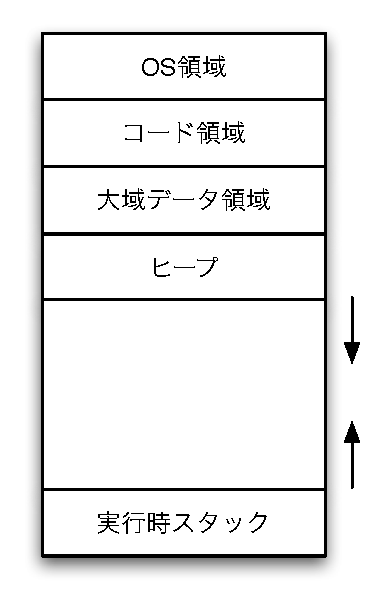
\includegraphics{figure/memory_area.pdf}
 \end{center}
 \caption{メモリ領域の分割例}
 \label{104220_11Apr06}
\end{figure}

ユーザ領域のうち、コード領域と大域データ領域の大きさはコンパイル時に決定
され、プログラム実行時には変化しない。一方、実行時スタックとヒープの大き
さは実行時に変化する。このような性質を満たすようなメモリ領域の使い方の一
例を図\ref{104220_11Apr06}に示す。この例では、メモリの下位番地からOS領域、
コード領域、大域データ領域、ヒープを割り当て、実行時スタックは逆にメモリ
の上位番地から割り当てる。

大域変数が割り当てられる番地はコンパイル時に決定される\footnote{現代のコ
ンピュータでは、複数のプログラムを同時に実行させることができる。そのため、
実際には、コード領域や大域データ領域についても、コード領域の先頭からの相
対番地のみ決定しておき、プログラム(機械語命令列)をメモリ上のどこにも配
置できるようにしておくことが多い。このような機械語命令列のことを
{\bfseries 再配置可能}(relocatable)であると言う。}。一方局所変数や実引
数は、プログラム実行中に関数が呼び出されたとき、実行時スタック上に割り当
てられるので、それまで番地は決定できない。また\icode{malloc()}などにより
動的に確保された領域も、実行時に実際にヒープに割り当てられるまで、番地は
決定できない。

\subsection{CPUとレジスタ}

メモリ上に配置された機械語プログラムはCPU(中央演算処理装置)が実行する。
具体的には、機械語プログラムを順に1命令ずつ読み出し、その命令に書かれた指
示に従ってメモリ領域やレジスタから値を読み出して算術演算や比較演算を行い、
結果をメモリ領域やレジスタに格納する。これを繰り返す。

Pentiumプロセッサには、次のようなレジスタが用意されている。
\begin{enumerate}
 \item {\bfseries 汎用レジスタ}(general-purpose register)…算術演算や
       比較演算などの演算数として用いることのできるレジスタ。本講義での
       機械語命令には、\icode{\%eax}, \icode{\%ebx}, \icode{\%ecx},
       \icode{\%edx}などのレジスタの他、実行時スタックを操作するのに用い
       られる{\bfseries ベースポインタ}(base pointer)\icode{\%ebp}と
       {\bfseries スタックポインタ}(stack pointer)\icode{\%esp}がある。
 \item {\bfseries 条件フラグ}(condition flag)…比較命令の結果を格納する
       レジスタ。ゼロフラグ\icode{\%zf}や符号フラグ\icode{\%sf}などがある。
       本講義で扱う機械語命令では、比較命令が自動的に設定し、条件付きジャ
       ンプ命令が適切なフラグを自動的に参照する。したがって、機械語命令に
       明示的に現れることはない。
 \item {\bfseries 命令ポインタ}(instruction pointer)…{\bfseries プログ
       ラムカウンタ}(program counter)とも言う。CPUが次に実行すべき命令
       の格納番地を指すレジスタ。\icode{\%eip}という記法を用いる。この値
       も自動的に更新されるため、命令ポインタが機械語命令に明示的に現れる
       ことはない。
\end{enumerate}

\subsection{機械語命令}

以降の説明を理解するのに必要な機械語命令について、簡単にまとめておく。な
お、本講義では Pentium プロセッサの機械語を記述するのに、AT\&T形式と呼ば
れるアセンブリ言語を用いている。

個々の機械語命令は、次のような書式をしている。[]は、その部分が省略可能で
あることを表している。
\begin{quote}
 [ラベル:] 命令名 第1演算数[, 第2演算数, $\cdots$, 第$n$演算数]
\end{quote}

ラベルは、コード領域中でこの機械語命令が置かれている番地を表すためのシン
ボルであり、先頭が\icode{\underline{ }}であるような文字列を用いる。関数に
相当する機械語命令列の先頭には、\icode{\underline{ }関数名}というラベルが
必ず付けられる。なお、図\ref{143232_11Apr06}の3行目のように、ラベルだけが
1行に書かれていても構わない。

演算数として用いることのできるのは、汎用レジスタ、メモリ番地、整数定数の
みである\footnote{整数定数以外の定数(文字列、浮動小数点数など)は、コー
ド領域や大域データ領域などに値を格納しておき、その番地をラベルで参照す
る。}。メモリ番地の指定は、以下の2通りの方法がある。
\begin{enumerate}
 \item その番地に付けられたラベル名
 \item 汎用レジスタの値を番地と見なし、その番地からの相対番地を指定する。
       例えば、$(レジスタRの値)$番地を$(\%R)$、$(レジスタRの値 + n)$番地
       を$n(\%R)$というように記述する。括弧がつくことで、レジスタそのもの
       ではなく、レジスタの値の番地という意味になることに注意してほしい
       \footnote{間接参照という。}。
\end{enumerate}
また整数定数の先頭には\$を付ける。

本講義では、実際の Pentium プロセッサの機械語のうちごく一部だけを用いる。
\begin{description}
 \item[2項算術命令] 演算数を2つとる算術演算。\icode{addl}(加算),
	    \icode{subl}(減算), \icode{imull}(乗算)などがある。結果は
	    第2演算数に格納される。例えば\icode{add~\%ebx,\%eax}は、レジ
	    スタ\icode{\%ebx}の値をレジスタ\icode{\%eax}の値に加え、結果
	    をレジスタ\icode{\%eax}に格納する。
 \item[単項算術命令] 演算数を1つとる算術演算。\icode{neg}(符号の反転)、
	    \icode{dec}(1引く)、\icode{inc}(1足す)などがある。結果は
	    第1演算数に格納される。例えば\icode{inc~\%eax}は、レジスタ
	    \icode{\%eax}の値に1を加え、結果を\icode{\%eax}に格納する。
 \item[移動命令] 演算数を2つとり、第1演算数の値を第2演算数に格納する。本
	    講義では\icode{movl}のみ扱う。例えば\icode{movl~\%eax,\%ebx}
	    は、レジスタ\icode{\%eax}の値をレジスタ\icode{\%ebx}に格納す
	    る。
 \item[比較命令] 演算数を2つとり、第1演算数と第2演算数を比較し、結果を条
	    件フラグに設定する。定数は第1演算数でのみ使える。本講義では
	    \icode{cmpl}のみ用いる。例えば\icode{cmpl~\$4,\%eax}は、定数4と
	    レジスタ\icode{\%eax}の値とを比較し、次のように条件フラグを設
	    定する。
	    \begin{align*}
	     {\sf zf}=0, {\sf sf=0} &&& 4<{\sf \%eax}のとき \\
	     {\sf zf}=1, {\sf sf=0} &&& 4={\sf \%eax}のとき \\
	     {\sf zf}=0, {\sf sf=1} &&& 4>{\sf \%eax}のとき
	    \end{align*}
 \item[無条件ジャンプ命令] \icode{jmp}命令。第1演算数にラベルをとり、その
	    ラベルの番地にジャンプする。実際には、ラベルの番地を命令ポイ
	    ンタ\icode{\%eip}に格納する、という動作をする。これにより、ラ
	    ベルの番地の機械語命令が次に実行されることになる。
 \item[条件ジャンプ命令] 第1演算数にラベルをとる。必ず比較命令と対にして
	    使われる。現在の条件フラグの値を参照し、ジャンプ条件と一致す
	    ればラベルの番地にジャンプする。一致しなければ次の命令に進む。
	    例えば\icode{jge}という条件ジャンプ命令は、${\sf sf}=0$のとき、
	    すなわち直前の比較命令で$第1演算数 \leq 第2演算数$であったと
	    きにジャンプする。条件ジャンプ命令と、そのジャンプ条件を以下
	    にまとめておく。($x, y$はそれぞれ第1演算数、第2演算数を表す)
	    \begin{align*}
	     {\sf jg} &&& {\sf zf}=0 \wedge {\sf sf}=0 & (x < y)\\
	     {\sf jge} &&& {\sf sf}=0 & (x \leq y)\\
	     {\sf je} &&& {\sf zf}=1 & (x = y)\\
	     {\sf jne} &&& {\sf zf}=0 & (x \neq y)\\
	     {\sf jl} & & & {\sf sf}=1 & (x > y)\\
	     {\sf jle} & & & {\sf zf}=1 \vee {\sf sf}=1 & (x \geq y)
	    \end{align*}
 \item[実行時スタック操作命令] 実行時スタックの一番上の番地はスタックポイ
	    ンタ\icode{\%esp}に格納されている。この値を変更し、実行時スタッ
	    クに要素を積んだり(\icode{push}命令)、先頭の要素をおろした
	    り(\icode{pop}命令)する命令である。図\ref{104220_11Apr06}で
	    分かる通り、番地の下位方向に実行時スタックが伸びることに注意
	    しておいてほしい。したがって、例えば\icode{push~\%eax}は、レ
	    ジスタ\icode{\%eax}の値を実行時スタックの一番上に積み、
	    \icode{\%esp}の値を1要素分、すなわち4減らす\footnote{ここでは
	    1要素が32ビット、すなわち4バイトであると仮定している。}。逆に
	    \icode{pop~\%ebx}は、実行時スタックの先頭の要素の値をレジスタ
	    \icode{\%ebx}に格納し、\icode{\%esp}の値を4増やす。
 \item[関数呼び出し命令] \icode{call}命令。第1演算数に関数を表すラベルを
	    指定し、その関数を呼び出す。次節で詳しく説明する。
 \item[関数からの戻り命令] \icode{ret}命令。関数の実行を終了し、関数呼び
	    出し前の番地に制御を移す。次節で詳しく説明する。
\end{description}

\section{関数の呼び出し}
\label{181902_17Apr06}

関数呼び出しの際には、考慮しなければならない点がいくつもある。説明のため、
\icode{main}関数から\icode{foo}関数を呼び出すとする。
\begin{itemize}
 \item \icode{foo}を呼び出す前に、実引数を設定しなければならない。これは
       \icode{main}側で行われる作業であり、かつ実行時スタックを用いなけれ
       ばならない。
 \item \icode{foo}の終了時に返り値を設定し、\icode{main}に渡さなければな
       らない。
 \item \icode{foo}の実行を始める前に、局所変数の領域を実行時スタックに確
       保し、必要なら初期化を行わなければならない。
 \item \icode{foo}を呼び出す前と\icode{foo}を呼び出した後で、レジスタや実
       行時スタックの状態は変化してはならない(返り値の設定を除く)
       \footnote{大域データ領域やヒープは変化しても構わない。}。つまり、
       \icode{foo}を呼び出す前に汎用レジスタ、命令ポインタ、スタックポイ
       ンタ、ベースポインタなどの内容を実行時スタックに退避し、
       \icode{foo}の終了時に退避した内容を適切に復帰しなければならない。
\end{itemize}

実際の機械語命令を見ながら、関数呼び出しのときに何が起こるか説明する。次
のような非常に簡単なCプログラムを考える。

\begin{quote}
 \lstinputlisting{code/foo.c} 
\end{quote}

この関数を\icode{main}から呼び出す場合、次のようなCプログラムになるだろ
う。

\begin{quote}
 \lstinputlisting{code/callfoo.c}
\end{quote}

さて、関数\icode{foo}に対応する機械語命令列は次のようになる(必要部分のみ
抜粋)。

\begin{quote}
 \lstinputlisting[language={[x86masm]Assembler},numbers=left,firstline=3,lastline=14]{code/foo.s}
\end{quote}

また、\icode{main}側で\icode{foo}を呼び出す部分は、次のような機械語命令列
になる(必要部分のみ抜粋)。

\begin{quote}
 \lstinputlisting[language={[x86masm]Assembler},numbers=left,firstline=7,lastline=8]{code/callfoo.s}
\end{quote}

\begin{figure}
 \begin{center}
  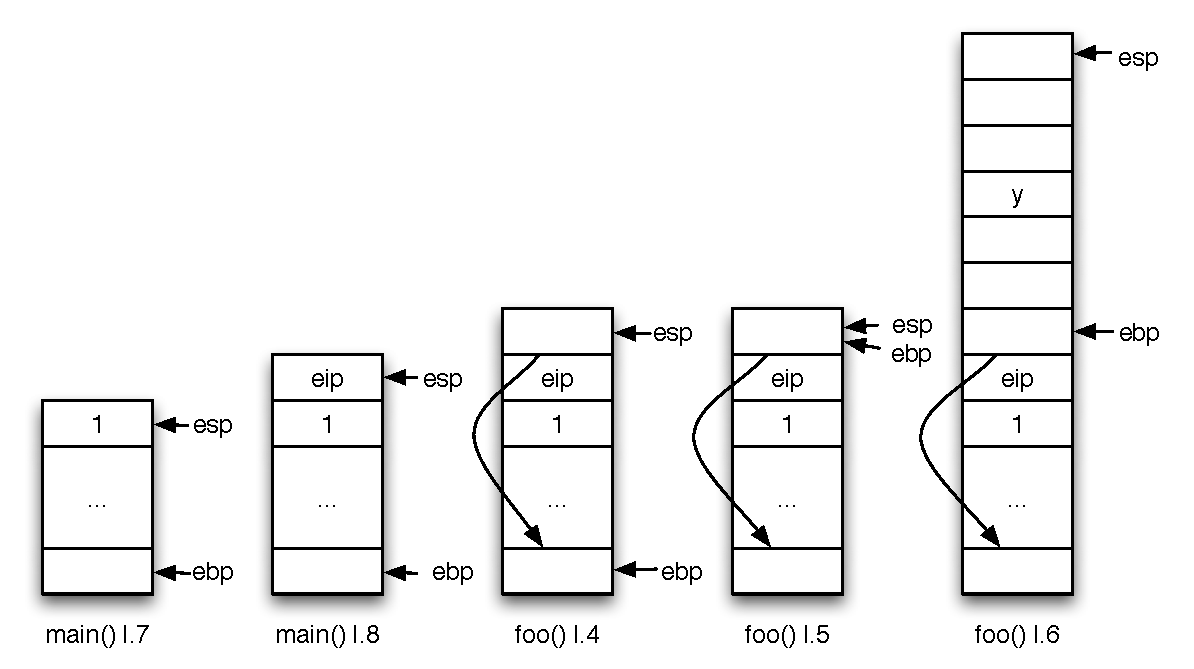
\includegraphics[width=12cm]{figure/function_call.pdf}
 \end{center}
 \caption{関数\icode{foo}呼び出し時の実行時スタック管理}
 \label{185859_11Apr06}
\end{figure}

\icode{foo}を呼び出すとき、\icode{foo}の終了時それぞれについて、上に示し
た機械語命令を追っていこう。まず\icode{foo}の呼び出し時である(図
\ref{185859_11Apr06})。
\begin{enumerate}
 \item \icode{main}の7行目: 実引数の設定。\icode{(\%esp)}、すなわちスタッ
       クポインタの指し示している実行時スタック領域(実行時スタックの先頭)
       に1を格納する。これが$x$に対応する実引数になる\footnote{ここでは示
       していないが、6行目以前では、実行時スタックの先頭には何も値が格納
       されていない。したがって、実行時スタックの先頭の値が上書きされるこ
       とはない。}。
 \item \icode{main}の8行目: \icode{foo}関数の呼び出し。\icode{call}命令で
       は、(命令ポインタ\icode{\%eip}の値$+1$)が実行時スタックにプッシュ
       され(\icode{\%eip}の退避)、\icode{\_foo}ラベル、すなわち関数
       \icode{foo}の3行目の番地が\icode{\%eip}に格納される。したがって、
       次に実行される機械語命令は\icode{foo}の3行目になる。
       \label{181636_11Apr06}
 \item \icode{foo}の3行目: ラベルだけなので、何も行われない。
 \item \icode{foo}の4行目: ベースポインタ\icode{\%ebp}の現在の値、すなわ
       ち\icode{foo}呼び出し前のベースポインタの値を実行時スタックにプッ
       シュする。(\icode{\%ebp}の退避)
       \label{181349_11Apr06}
 \item \icode{foo}の5行目: スタックポインタ\icode{\%esp}の現在の値を
       \icode{\%ebp}に格納する。これにより、\icode{foo}の実行に入る前のス
       タックポインタの値がベースポインタ\icode{\%ebp}に退避されたことに
       なる。(\icode{\%esp}の退避)
       \label{181051_11Apr06}
 \item \icode{foo}の6行目: スタックポインタ\icode{\%esp}の値を24減らす。
       これは、実行時スタックに要素を6個積んだことに相当している。この中
       には、局所変数$y$の領域\footnote{\icode{-12(\%ebp)}、すなわちこの時
       点でのベースポインタから3要素分上の領域である。}なども含まれてい
       る。
 \item \icode{foo}の7-9行目: 局所変数$y$の初期化。実引数$x$の領域は
       \icode{8(\%ebp)}、つまりこの時点でのベースポインタから2要素分下の
       領域であることに注意せよ。
\end{enumerate}

\begin{figure}
 \begin{center}
  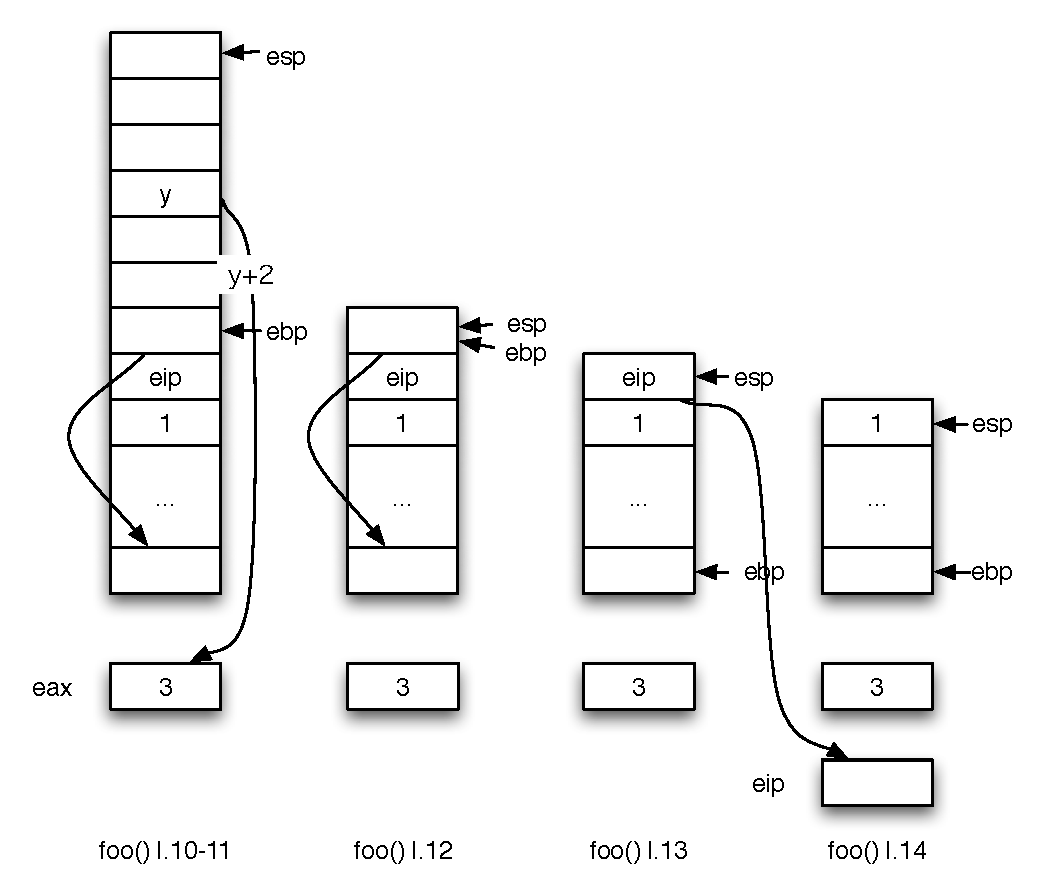
\includegraphics[width=12cm]{figure/function_return.pdf}
 \end{center} 
 \caption{関数\icode{foo}からの戻り処理}
 \label{191124_11Apr06}
\end{figure}

次に関数\icode{foo}の終了時の処理を追ってみる(図\ref{191124_11Apr06})。

\begin{enumerate}
 \item \icode{foo}の10-11行目: 返り値の設定。Pentiumプロセッサでは通常、
       関数からの返り値は汎用レジスタ\icode{\%eax}を使って、呼び出し元に
       受け渡される。ここでも、$y+2$の計算結果が\icode{\%eax}に格納されて
       いる。
 \item \icode{foo}の12行目: 現在のベースポインタ\icode{\%ebp}の値をスタッ
       クポインタ\icode{\%esp}に格納する。呼び出し時の処理
       \ref{181051_11Apr06}で、呼び出し前のスタックポインタの値を
       \icode{\%ebp}に退避していたことに注意せよ。つまり、ここで
       \icode{\%esp}を呼び出し前の状態に復帰している。
 \item \icode{foo}の13行目: 実行時スタックの先頭の要素をポップし、ベース
       ポインタ\icode{\%ebp}に格納している。呼び出し前の処理
       \ref{181349_11Apr06}で、呼び出し前のベースポインタの値を実行時スタッ
       クに退避していたことに注意せよ。つまり、ここで\icode{\%ebp}を呼び
       出し前の状態に復帰している。
 \item \icode{foo}の14行目: \icode{foo}関数からの戻り。\icode{ret}命令で
       は、実行時スタックの先頭の要素をポップし、命令ポインタ
       \icode{\%eip}に格納する。呼び出し前の処理\ref{181636_11Apr06}で、
       呼び出し前の\icode{\%eip}の値を実行時スタックに退避していたことに
       注意せよ。つまり、ここで\icode{\%eip}を呼び出し前の状態に復帰して
       いる。したがって、次の機械語命令は\icode{call}命令の番地$+1$、すな
       わち\icode{call}命令の次の機械語命令になる。
\end{enumerate}

関数呼び出し時、および関数終了時には、常に上記のような処理が行われる。た
だし実際には、他の汎用レジスタの退避・復帰のための機械語命令列も加えられ
ることがある。
